\documentclass[default,iicol]{sn-jnl}

\usepackage{amsmath}
\usepackage{array}
\usepackage[acronym]{glossaries}
\usepackage{epsfig} %% for loading postscript figures
\usepackage{float}
\usepackage[utf8]{inputenc}
\usepackage{siunitx}
\usepackage{stfloats}
\usepackage{subfig}
\usepackage{titlesec}
\usepackage{url}
\usepackage{xcolor}


% get rid of colon for tables and figures as requested per journal format
\usepackage[labelsep=space]{caption}

\setcounter{secnumdepth}{4}

\titleformat{\paragraph}
{\normalfont\normalsize\bfseries}{\theparagraph}{1em}{}
\titlespacing*{\paragraph}
{0pt}{3.25ex plus 1ex minus .2ex}{1.5ex plus .2ex}

%\def\url#1{\expandafter\string\csname #1\endcsname}
\newcounter{exno}
\newenvironment{examples}
{
\begin{flushleft}
\begin{tabular}{>{(\refstepcounter{exno}\theexno\label{row:\theexno}) }rl}
}
{
\end{tabular}
\end{flushleft}
}
%\newcommand*{\@rowstyle}{}
\newcommand*{\rowstyle}[1]{% sets the style of the next row
  \gdef\@rowstyle{#1}%
  \@rowstyle\ignorespaces%
}
\newcolumntype{=}{% resets the row style
  >{\gdef\@rowstyle{}}%
}
\newcolumntype{+}{% adds the current row style to the next column
  >{\@rowstyle}%
}
\definecolor{ao}{rgb}{0.0, 0.5, 0.0}
\definecolor{coolblack}{rgb}{0.0, 0.18, 0.39}

\glsdisablehyper
\newacronym[longplural={centers of mass}]{com}{CoM}{center of mass}
\newacronym[longplural={equations of motion}]{eom}{EoM}{equation of motion}
\newacronym{ocp}{OCP}{optimal control problem}
\newacronym{nlp}{NLP}{non-linear programming problem}
\newacronym[longplural={degrees of freedom}]{dof}{DoF}{degree of freedom}

\newcounter{magicrownumbers}
\newcommand\rownumber{\stepcounter{magicrownumbers}\arabic{magicrownumbers}}
\newcommand\figwidth{174mm}

\jyear{2021}%

\raggedbottom
%%\unnumbered% uncomment this for unnumbered level heads

\begin{document}


\title[Maximizing Ollie Height by Optimizing Control Strategy and Skateboard Geometry Using Direct Collocation]{
  Maximizing Ollie Height by Optimizing Control Strategy and Skateboard Geometry Using Direct Collocation}

%%=============================================================%%
%% Prefix	-> \pfx{Dr}
%% GivenName	-> \fnm{Joergen W.}
%% Particle	-> \spfx{van der} -> surname prefix
%% FamilyName	-> \sur{Ploeg}
%% Suffix	-> \sfx{IV}
%% NatureName	-> \tanm{Poet Laureate} -> Title after name
%% Degrees	-> \dgr{MSc, PhD}
%% \author*[1,2]{\pfx{Dr} \fnm{Joergen W.} \spfx{van der} \sur{Ploeg} \sfx{IV} \tanm{Poet Laureate} 
%%                 \dgr{MSc, PhD}}\email{iauthor@gmail.com}
%%=============================================================%%

\author[1]{\fnm{Jan T.} \sur{Heinen}}\email{janheinen97@gmail.com}

\author[1]{\fnm{Samuel G.} \sur{Brockie}}\email{s.g.brockie@tudelft.nl}

\author[2]{\fnm{Raymund} \sur{ten Broek}}\email{raymund@uspc.nl}

\author[1]{\fnm{Eline} \sur{van der Kruk}}\email{e.vanderkruk@tudelft.nl}

\author*[1]{\fnm{Jason K.} \sur{Moore}}\email{j.k.moore@tudelft.nl}

\affil*[1]{\orgdiv{Department of Biomechanical Engineering}, \orgname{Delft University of Technology}, \orgaddress{\street{Mekelweg}, \postcode{2628 CN}, \city{Delft}, \country{The Netherlands}}}
\affil*[2]{\orgname{Urbansports Performance Centre}, \orgaddress{\street{Veemstraat}, \postcode{5617 AG}, \city{Eindhoven}, \country{The Netherlands}}}

\abstract{The ollie is the base aerial human-board maneuver, foundational to most modern skateboarding tricks. We formulate and solve an optimal control problem of a two-dimensional simplified human model and a rigid body skateboard with the objective of maximizing the height of the ollie. Our solution simultaneously discovers realistic human-applied force trajectories and optimal board geometry. We accomplish this with a direct collocation formulation using a null seed initial guess by carefully modeling the discontinuous aspects of board-ground impact and foot-board friction. This leads to very efficient and robust solutions that are 10 times more computationally efficient than prior work on similar problems. The solutions show that ollie height can increase 3\% by decreasing the wheelbase and that a smaller board with a back-foot dominated force strategy can give 12\% higher ollies. Our model can be used to inform jump strategy and the effects of changes to the essential board geometry.}

\keywords{Skateboarding, Friction, Impact, Optimal Control, Trajectory Optimization, Parameter Optimization, Direct Collocation}
\maketitle

\section{Introduction}\label{s_intro}

In 1978 Alan `Ollie' Gelfand invented the `no-hand aerial', by riding off an inclined surface and jumping in the air with a skateboard.
Four years later, Rodney Mullen debuted the first ollie from flat ground.
Because the skateboard is not tethered to the skater, an ollie requires a precise sequence of movements to keep the two together~\cite{frederick_biomechanics_2006}.
The maneuver can be deconstructed into the six
distinct phases shown in Fig.~\ref{fig:ollie steps}.

\begin{figure*}[!t]
\captionsetup[subfigure]{labelformat=empty}
  \subfloat[$t_1$=0.013]{{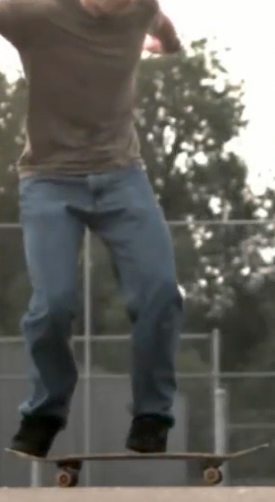
\includegraphics[width=0.13\textwidth]{figure/Fig1a.png} }}%
  \subfloat[$t_2$=0.129]{{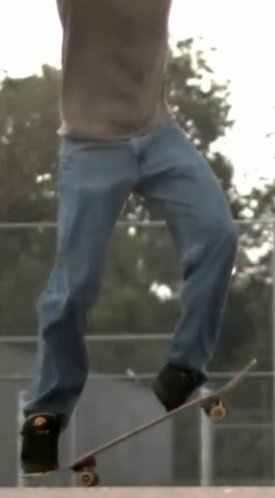
\includegraphics[width=0.13\textwidth]{figure/Fig1b.png} }}%
  \subfloat[$t_3$=0.181]{{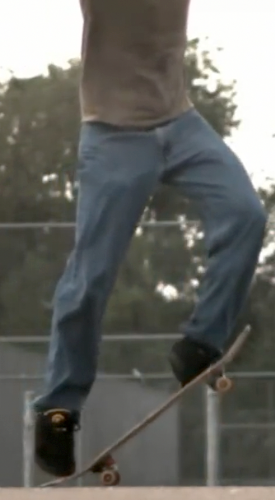
\includegraphics[width=0.13\textwidth]{figure/Fig1c.png} }}%
  \subfloat[$t_4$=0.187]{{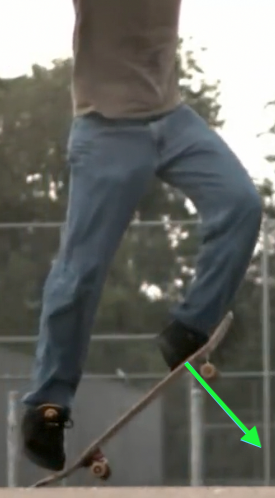
\includegraphics[width=0.13\textwidth]{figure/Fig1d.png} }}%
  \subfloat[$t_5$=0.303]{{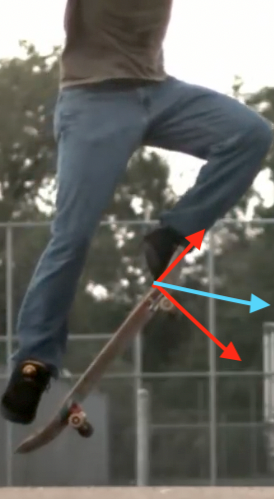
\includegraphics[width=0.13\textwidth]{figure/Fig1e.png} }}%
  \subfloat[$t_6$=0.431]{{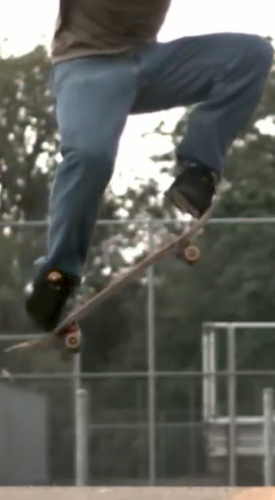
\includegraphics[width=0.13\textwidth]{figure/Fig1f.png} }}%
  \subfloat[$t_7$=0.543]{{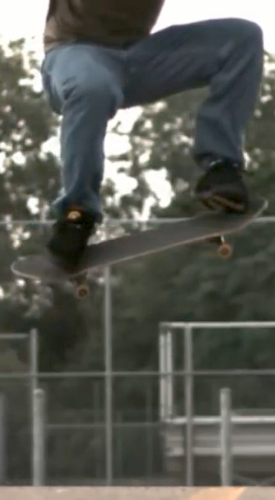
\includegraphics[width=0.13\textwidth]{figure/Fig1g.png} }}%
  \protect\newline
  \centering
  \subfloat[$t_8$=0.676]{{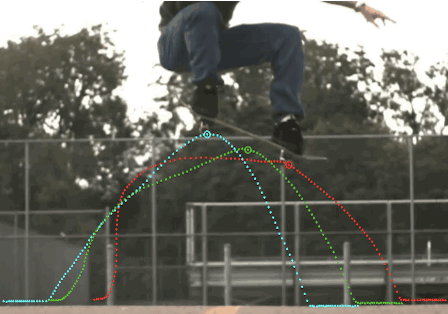
\includegraphics[width=0.336\textwidth]{figure/Fig1h.png} }}
  \subfloat[$t_9$=0.722]{{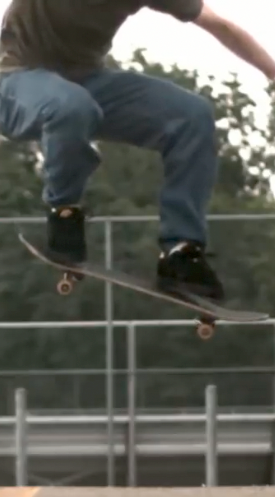
\includegraphics[width=0.13\textwidth]{figure/Fig1i.png} }}%
  \subfloat[$t_{10}$=0.904]{{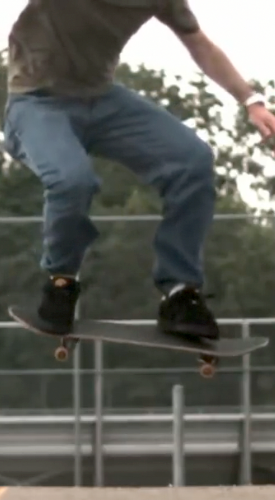
\includegraphics[width=0.13\textwidth]{figure/Fig1j.png} }}%
  \subfloat[$t_{11}$=1.097]{{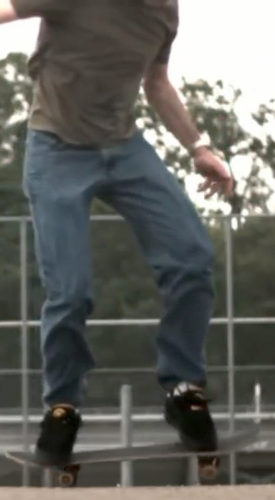
\includegraphics[width=0.13\textwidth]{figure/Fig1k.png} }}%
  \captionsetup{singlelinecheck=off}
   \caption[Ollie motion cues]{Phases of the ollie.
    Green arrow: resultant force without friction, red arrows: force components
    with friction, blue arrow: resultant force with friction. Blue-, green- and
    red lines are trajectory of back wheel, middle and front wheel respectively. Images are retrieved from \url{youtu.be/339k4XEvbxY} with consent. The phases and associated motion cues are described by:\\
    \begin{center}
    \begin{tabular}{p{1.6cm} p{0.3cm} p{12.7cm}}
        Preparation     & $t_1$ & The skater lowers their \gls{com} preparing to jump \\
        Pre-pop         & $t_2$ & The skater pushes firmly from their back leg and is decreasing downward force on the front foot, which results in the front wheels leaving the ground, simultaneously sliding the front foot forward \\
        Pop             & $t_3$ & Tail collides with the ground, the front foot is still sliding and the back foot is barely in contact with the skateboard~\cite{determan_kinetics_2006,nakashima_simulation_2021} \\
        Upward motion   & $t_4$ & Back foot is no longer in contact with the skateboard, the back wheels are not in contact with the ground anymore~\cite{determan_kinetics_2006,nakashima_simulation_2021} \\
                        & $t_5$ & The front foot reached the nose of the skateboard \\
                        & $t_6$ & Back foot contacts the board again \\
                        & $t_7$ & Board is leveled out by the front foot \\
                        & $t_8$ & Highest point is reached. Knees are fully tucked in, touching the chest, restricting the board from gaining height. Feet are firmly placed on the deck \\
        Downward motion & $t_9$ & Front foot loses contact \\
                        & $t_{10}$& Board is horizontal, both feet are in contact \\
        Landing         & $t_{11}$& The back wheels touch the ground and legs are almost fully stretched out \\
    \end{tabular}
    \end{center}
}
  \label{fig:ollie steps}
\end{figure*}

From the early 1960s, new skateboarding pursuits and their differing performance requirements evolved a variety of skateboard shapes.
For example, slalom demanded short boards for quick turns, downhill preferred longboards for stability, and pool skating resulted in wide, concave boards for maximum foothold. 
Artistic motives shaped impractical coffin- and
fish-like boards~\cite{prentiss_get_2011}.
The prevailing modern board shape, used by all Olympic athletes, is the popsicle stick.
The shape supports a variety of freestyle aerial tricks, where the ollie is the foundational aerial maneuver.
A labeled diagram of a popsicle stick skateboard is shown in Fig.~\ref{fig:skateboard terminology} (the skateboard front and riding direction will always be in the positive x-direction).

Friction occurs between the feet and the board surface due to the normal force exerted by the feet together with sliding movement tangential to the board's surface which is covered by griptape (sandpaper).
This benefits ollie height because the resultant force (Fig.~\ref{fig:ollie steps} $t_5$, blue arrow) is directed more vertically upwards than the normal force (Fig.~\ref{fig:ollie steps} $t_4$, green arrow), which results in less downward motion while leveling out the skateboard mid-air.
The higher the coefficient of friction between the foot and the deck, the more upward the resultant force will be.
That is why griptape on the deck and rubber-soled shoes are preferred by skaters.

Impact is also important in the mechanics of an ollie.
An impulsive impact between the tail and the ground causes the `pop', which changes the translational and angular velocities of the board, causing it to lose contact with the ground and move upwards.

There is no standardization of popsicle stick boards in the skateboard industry.
Boards are measured differently by each brand~\cite{johnny_skateboarding_2013} and non-specific descriptions such as mellow, steep, and wide are usually used to communicate deck dimensions to customers~\cite{berger_handmade_2021}.
This makes it difficult for skaters to find their optimal board shape.

Skaters know and feel when a specific skateboard performs to their liking.
However, they do not know how this translates to quantifiable board dimensions.
Skateboards might have evolved to optimum geometries over the years, but from an academic and mechanical point of view, skateboard designs have not been shown to be optimal for specific tricks.

Researchers have analyzed the skateboard in planar riding models~\cite{hubbard_lateral_1979,kremnev_nonlinear_2010,varszegi_stability_2017}, which show the relationship between the dimensions and the stability while rolling and turning. 
However, these dimensional analyses do not apply to aerial movements like the ollie.
Others research the ollie by investigating the simulated contact forces~\cite{anderson_ollie_2020,shield_contact-implicit_2022} and through experimental biomechanics~\cite{frederick_biomechanics_2006,vorlicek_analysis_2015,wood_3d_2020,candotti_lower_2012,dias_using_2016}.
\citet{shield_contact-implicit_2022} and \citet{anderson_ollie_2020} found optimal ollie motions without changing the geometry, but no research has yet shown how the skateboards' dimensions influence ollie height.

Now that skateboarding is an Olympic sport, knowing how to improve performance is more important than ever.
Achieved height is the most measurable Olympic judging criteria applicable to the ollie~\cite{world_skate_skateboarding_2021}.
This leads to our research question:
\begin{quote}
\textit{
    What are the optimal geometric parameters of a skateboard for an athlete to reach maximal ollie height?}
\end{quote}
We find answers to this question by formulating a simple human-skateboard dynamics model and solving an \gls{ocp} utilizing direct collocation methods.

\begin{figure}[t]
    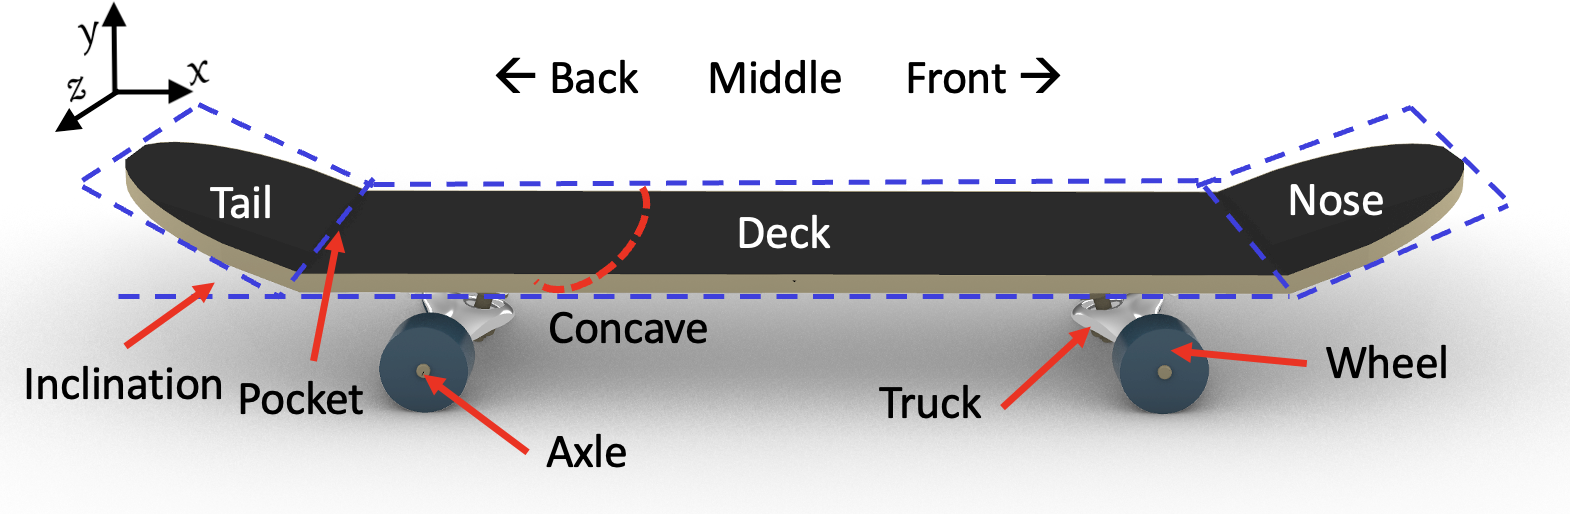
\includegraphics[width=0.5\textwidth]{figure/Fig2.png}
    \caption[Skateboard terminology]{Skateboard terminology}
    \label{fig:skateboard terminology}
\end{figure}

\section{Method}

\subsection{Skateboard Equations of Motion}
We start by developing a simple 2D rigid body model of the skateboard.
The board was modelled as a simplified popsicle stick skateboard with an assumption about nose-tail symmetry and no deck concavity.
While in reality a skateboard bends and flexes during the ollie, this study assumed a rigid body model of the skateboard to reduce mathematical complexity.

The skateboard model is detailed in Fig.~\ref{fig:FBD}. During wheel-ground contact, we use a sliding joint for the rear wheel contact to eliminate the ground reaction forces from the \glspl{eom}.
When the board is airborne during the ollie, we treat the skateboard as an unconstrained rigid body in 2D. 

\begin{figure}
    \centering
    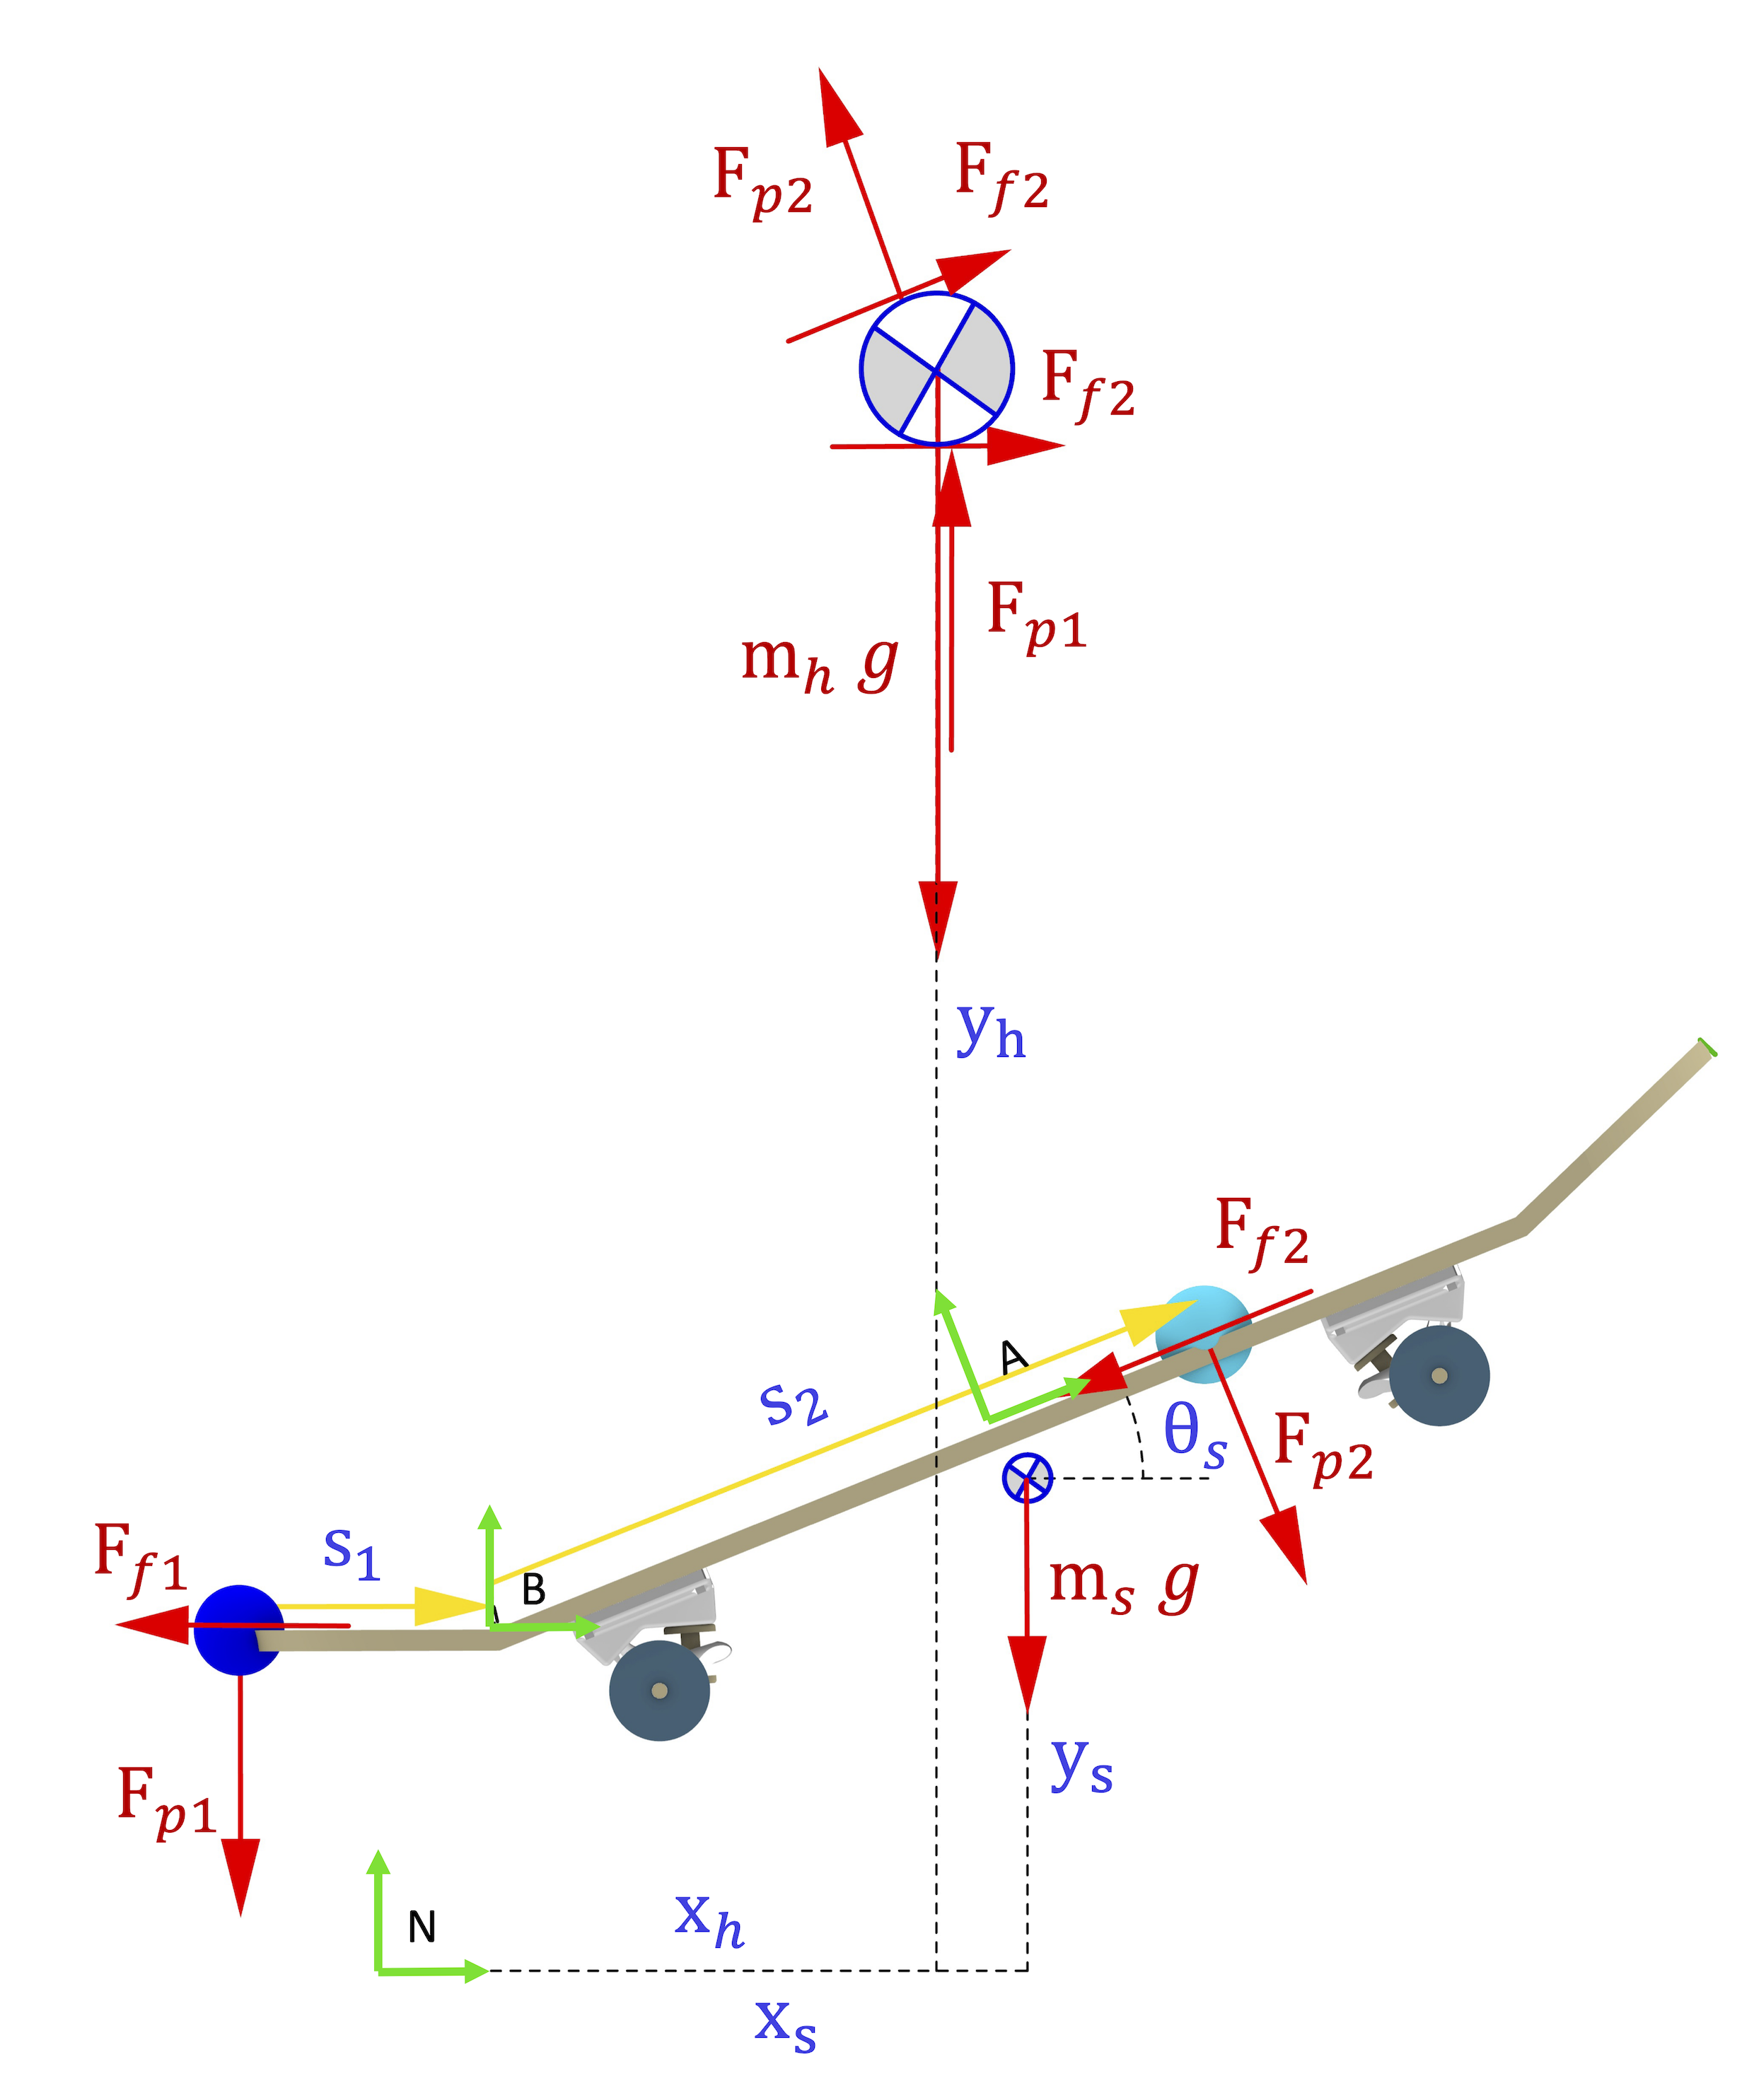
\includegraphics[width=0.45\textwidth]{figure/Fig3.png}
    \footnotesize
  \begin{center}
  \begin{tabular}{l c}
    \toprule
    \color{blue}Blue: & State variables \\
    \color{red} Red: & Forces \\ 
    \color{cyan}Cyan dot: & Front foot \\
    \color{blue}Blue dot: & Back foot \\ 
    \color{yellow}Yellow: & Foot movement \\
    \color{green}Green: & Frames \\
    \bottomrule
    \end{tabular}
    \end{center}
    
    % \footnotesize\begin{tabular}{|l l|l l|} \hline
    % \color{blue}Blue: & State variables &\color{red} Red: & Forces \\ \hline
    % \color{cyan}Cyan dot: & Front foot & \color{blue}Blue dot: & Back foot \\ \hline
    % \color{yellow}Yellow: & Foot movement & \color{green}Green: & Frames \\ \hline
    % \end{tabular}
    \caption[Free Body Diagram of Phase 1]{Free body diagrams of human and skateboard. $N$ is the inertial reference frame, and $A$ and $B$ are skateboard-fixed reference frames. Forces acting between the foot locations on the board and human's \gls{com} ($F_{f1}$, $F_{p1}$, $F_{f2}$, $F_{p2}$) are equal and opposite. $x_s$, $y_s$, $x_h$, and $y_h$ locate the skateboard and human in $N$. $\theta_s$ is the skateboard's inclination angle. $s_1$ and $s_2$ are the positions of the back and front foot on the board. $g$ is the acceleration due to gravity. $m_h$ and $m_s$ are the mass of the human and skateboard, respectively}
    \label{fig:FBD}
\end{figure}

\subsection{Athlete Equations of Motion}
The athlete was modeled as a point mass with a mass of \SI{80}{\kilo\gram} and no rotational inertia (Fig.~\ref{fig:FBD}).
The contact forces between the point mass and the skateboard were modeled as a pair of equal and opposite forces acting between the massless feet and the athlete's \acrfull{com}.
Due to this simplification, this does not model metabolic leg power, only the mechanical power output~\cite{van_der_kruk_power_2018,morin_biomechanics_2018}.

We derived the \glspl{eom} using the TMT method~\cite{vallery_heike_advanced_2018}, facilitated by SymPy~\cite{meurer_sympy_2017}.
The code used for the derivation is provided in \cite{heinen_optimal_2022}, along with a derivation of the \glspl{eom}.

Several kinetic and kinematic constraints were introduced to create a realistic simulation. Firstly, the feet are constrained to the surface of the board and can move only within a fixed region relative to the human’s \gls{com}: $\SI{0.466}{\meter} \leq y_h - y_{foot} \leq \SI{1.13}{\meter}$.

These bounds were found by scaling a human inertia model to \SI{1.80}{\meter} tall and posing it to match a picture of Jake Hayes' world record ollie  (Fig.~\ref{fig:f_record}) using the software Yeadon~\cite{Dembia2015}. 

\begin{figure}
    \centering
    \subfloat[\centering \SI{115.6}{\centi\meter} world record ollie.]{{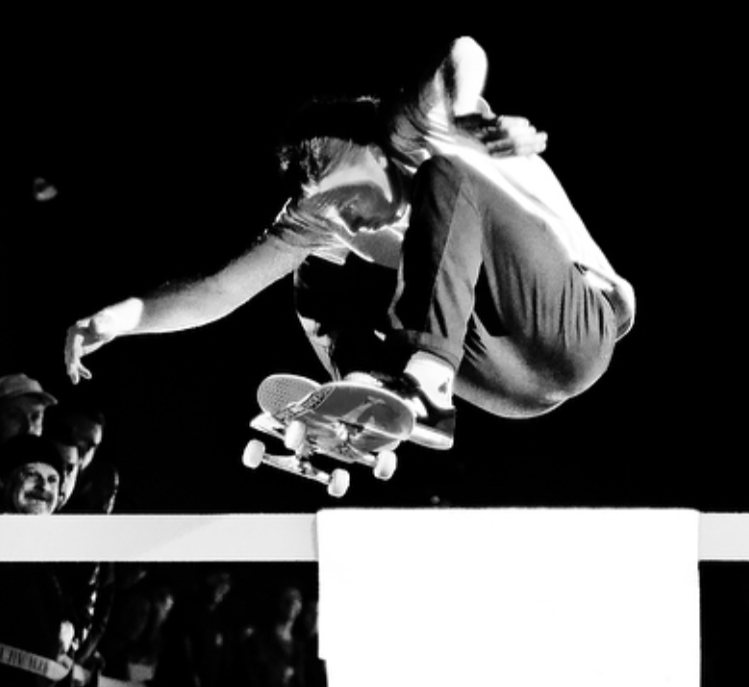
\includegraphics[width=0.2\textwidth]{figure/Fig4a.png} }}%
    \quad
    \subfloat[\centering Yeadon model in same configuration]{{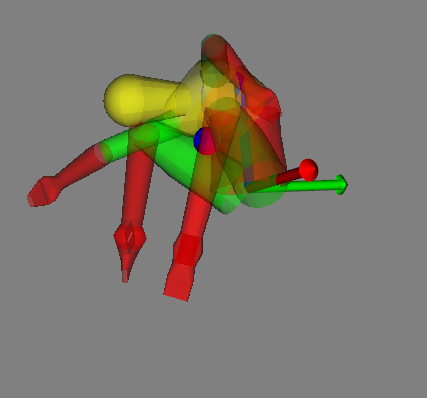
\includegraphics[width=0.2\textwidth]{figure/Fig4b.png} }}%
    \caption{Reconstruction of world record ollie} 
    \label{fig:f_record}
\end{figure}

We also implement a minimum and maximum foot-to-foot separation of \SI{0.1}{\meter} and \SI{1.0}{\meter}, respectively, along with constraining the skater to always stay on top of the skateboard to eliminate relative errors.
To make sure the feet never leave the skateboard, the rear foot is bound to the tail section and the front foot to the flat section of the deck (see Fig.~\ref{fig:FBD}).
The feet can disconnect from the board, as seen in Fig.~\ref{fig:ollie steps}, but due to how the friction model is implemented (section~\ref{ss_friction}).

We constrain the rate of force development to simulate the leg shortening and lengthening cycle, the maximum force $F_{max}$ to keep this within realistic limits, and maximum mechanical power $P = F v_{rel}$ as this also constrains knee extension rate. We obtained numerical values from a countermovement jump study that tested Division-I male soccer players with a mean height of \SI{179.5}{\centi\meter}, weight of \SI{75.5}{\kilo\gram}, and age of 19.65 years~\cite{barker_relationships_2018}. The kinetics of the human controls are bound to the characteristics of a countermovement jump motion because it accounts for 76.3\% of the variance in the performance of the ollie~\cite{candotti_lower_2012} and is a reliable assessor of lower-body mechanical power~\cite{barker_relationships_2018}. 

To account for the fact that \citet{barker_relationships_2018} measured two legs simultaneously, we constrain the sum of the forces produced by both legs together. We also constrain the absolute force and power produced by each leg to within realistic physical limits to prevent in and out-of-phase pushing and pulling of the individual legs.

\subsection{Friction and Impact Model} \label{ss_friction}
The feet slide along the deck's griptape to drag vertically and level the skateboard. We model both the static and dynamic friction during the foot's sliding on the deck using an approach based the relaxed formulation by \citet{patel_contact-implicit_2019}, which models implicit impact and friction.
Application of the relaxed formulation can result in slow convergence and long compute times and require a close initial guess~\cite{shield_contact-implicit_2022}. We chose to use a variation to this formulation with a simplified foot-board contact model and a multi-phase method for the tail-ground impact to have faster convergence and no need for a close initial guess.

We modify the relaxed formulation by removing the impact condition between the human and the board, instead assuming that the feet never impact the skateboard and simply exert zero normal force when out of contact.
We start by setting the normal forces of the feet $F_{p1}, F_{p2}$ and the feet accelerations $\ddot{s}_1, \ddot{s}_2$ as control variables.
Foot acceleration is controlled instead of foot location itself to ensure smooth and realistic foot trajectories.
We divide each normal force into a pair of non-negative slack variables representing its positive and negative component, for example, $F_{f1} = F_{f1}^+ - F_{f1}^-$.

Friction is then enforced using a set of six path constraints for each foot (shown below for the back foot):
\begin{align} \label{e_frictioncontrol}
    \psi_1 + \dot s_1  &\geq 0 \\
    \psi_1 - \dot s_1  &\geq 0 \\
    \mu F_{p1} - F_{f1}^+ - F_{f1}^- &\geq 0 \\
    (\mu F_{p1} - F_{f1}^+ - F_{f1}^-)\ \psi_1  &= 0 \\
    F_{f1}^+ (\psi_1 + \dot s_1)  &= 0 \\
    F_{f1}^- (\psi_1 - \dot s_1)  &= 0
\end{align}
The first two equations above introduce $\psi_1$, a slack variable representing the magnitude of the relative velocity between the foot and the skateboard $\dot{s}_1$. The third ensures that the positive or negative component of the friction is always smaller than $\mu F_{p1}$, while the fourth ensures that when the foot slides the sum of the positive and negative friction components equal $\mu F_{p1}$. It is important that when sliding in the positive direction, the negative friction component $F_{f1}^- = \mu F_{p1}$ and $F_{f1}^+=0$, and vice versa. This is enforced by the final two path constraints, (5) and (6).

The translational and angular velocities after tail-ground impact are calculated with the Newton impact law as presented in \citet{vallery_heike_advanced_2018} with a coefficient of restitution of $e=0.8$.

\subsection{Geometry and Parameterization}\label{s_paropt}
The skateboard model is described using ten variables. This includes six optimizable parameters: wheelbase ($l_{wb}$), deck length ($l_{d}$), tail/nose length ($l_{t}$), tail/nose inclination ($\phi$), truck height ($h_{tr}$), and wheel radius ($r_w$). Four additional parameters, which were dimensions orthogonal to the 2D plane of the model, were fixed to industry-standard values: deck thickness ($h_d = \SI{0.0012}{\meter}$), truck width ($d_{tr} = \SI{0.21}{\meter}$), deck width ($d_d = \SI{0.21}{\meter}$), and wheel width ($d_w = \SI{0.031}{\meter}$). The optimizable and fixed parameters are shown in Fig.~\ref{fig:parameterized skateboard} in blue and green respectively.

%%%%%%%%%%%%%%%% begin figure %%%%%%%%%%%%%%%%%%%
\begin{figure}
  \centerline{
    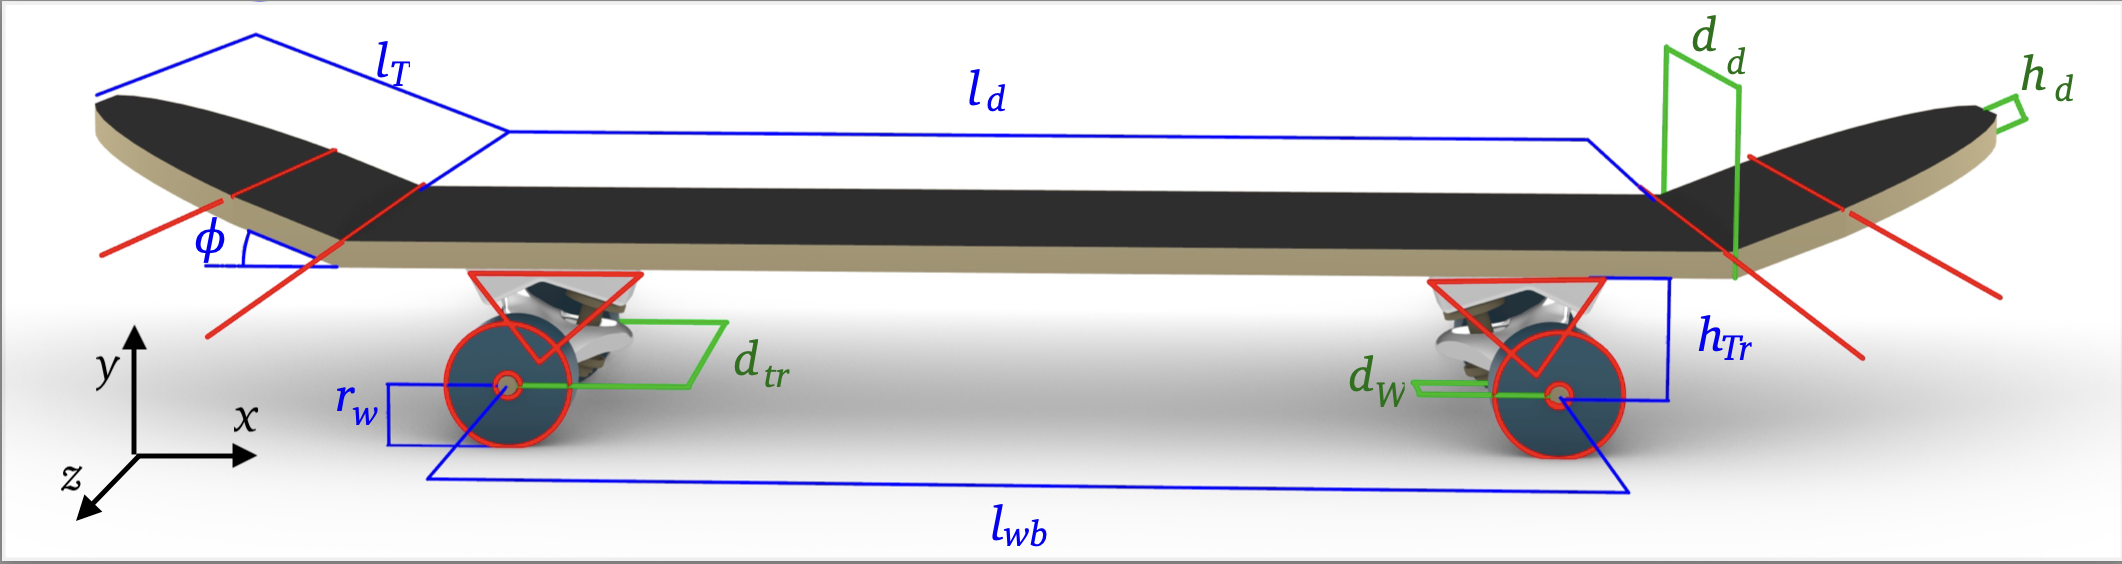
\includegraphics[width=0.5\textwidth,trim={0.1cm 0.1cm 0.1cm 0.05cm},clip]{figure/Fig5.png}
  }
  \footnotesize
  \begin{center}
  \begin{tabular}{=l +l +c}
    \toprule
    \rowstyle{\textbf}& Variable & Description \\
    \midrule
    \rowstyle{\color{blue}} & $l_{wb}$ & Wheelbase \\
    \rowstyle{\color{blue}} & $l_{d}$ & Deck length \\
    \rowstyle{\color{blue}} & $l_{t}$ & Tail/nose length \\
    \rowstyle{\color{blue}} & $\phi$ & Tail/nose inclination \\
    \rowstyle{\color{blue}} & $h_{tr}$ & Truck height \\
    \rowstyle{\color{blue}} & $r_{w}$ & Wheel radius \\
    \rowstyle{\color{ao}} & $h_d$ & Deck thickness \\
    \rowstyle{\color{ao}} & $d_{tr}$ & Truck width \\
    \rowstyle{\color{ao}} & $d_{d}$ & Deck width \\
    \rowstyle{\color{ao}} & $d_w$ & Wheel width \\
    \rowstyle{\color{orange}} & $d_{com}$ & CoM distance from deck \\
    \bottomrule
  \end{tabular}
  \end{center}
  \caption{Parameterized skateboard. Blue parameters are optimized, green parameters are set to industrial standards. Orange is dependent on other variables. Red lines split the skateboard into 11 basic shaped segments for inertia calculation}
\label{fig:parameterized skateboard}
\end{figure}
%%%%%%%%%%%%%%%% end figure %%%%%%%%%%%%%%%%%%%

The skateboard's mass and inertia were calculated as a composition of 11 simple constant-density 3D shapes (cuboidal, semicircular, and triangular prisms), shown in Fig.~\ref{fig:parameterized skateboard}, such that they were functions of the optimizable parameters. Material densities for wood, steel, and polyurethane of \SI{705}{\kilo\gram\per\meter\cubed}, \SI{7700}{\kilo\gram\per\meter\cubed}, and \SI{1130}{\kilo\gram\per\meter\cubed} respectively were used.

\subsection{Optimal Control Problem} \label{sec:ocp}
The \gls{ocp} was formulated with the objective of maximizing the peak board height during the ollie. The board dynamics, control, and geometric parameters are simultaneously optimized via trajectory optimization using a direct method.
The direct method is well suited for when dynamics and control must be computed to a similar accuracy and the structure of the control trajectory is not known a priori~\cite{kelly_introduction_2017}.

The \gls{ocp} was solved numerically using Pycollo~\cite{brockie_predictive_2021}. Pycollo solves the generalized multi-phase \gls{ocp} described in \citet{betts_practical_2010} by transcribing the \gls{ocp} to a \gls{nlp} using an LGL (Legendre-Gauss-Lobatto) collocation method~\cite{betts_using_2016}. The \gls{nlp} is then solved using Ipopt~\cite{biegler_large-scale_2009}. Pycollo uses ph-mesh refinement~\cite{patterson_ph_2015} to iteratively improve the transcription mesh, solving successive \glspl{nlp} until a desired solution tolerance is met.

\subsection{Phases} \label{s_phases}

The movement was divided into three dynamically-distinct sequential phases of flexible duration:
\begin{enumerate} \label{n_phases}
  \item Preparation phase (P1): P1 starts with the vertical forces equal to the body weight. The wheels are in contact with the ground throughout P1. P1 ends when the tail impacts the ground.
  \item Upward phase (P2): Neither wheel is in contact with the ground. The phase ends when the board's vertical velocity is zero.
  \item Downward phase (P3): This phase is governed by the same \glspl{eom} as P2. This phase and the \gls{ocp} terminate when one of the wheels touches the ground.
\end{enumerate}

We use a multi-phase formulation for the ollie \gls{ocp} to handle discontinuities in the state trajectories in a numerically-stable manner. This allows the impact of the tail with the ground during the pop to be treated as an impulse, which is not possible during a single continuous phase. It also allows a decision variable to be defined for the skateboard height at the end of P2, which is required in the objective function. A disadvantage of this approach is that the transition between phases is prescribed in terms of the system state, leaving no room for the optimizer to discover these transitions.

We used an initial transcription mesh involving 30 mesh sections for P1 and P2, and 10 mesh sections for P3. The optimal trajectory in P1 and P2 is more nonlinear than in P3 requiring a more dense mesh to be used.
Additionally, settings for the \gls{nlp} and mesh tolerances in Pycollo were set to $1e^{-8}$ and $1e^{-3}$ respectively.

\subsection{Objective Function}

The objective function for maximization is:
%
\begin{equation}
  \mathcal{J} = y_s^{(2)}\left(t_F^{(2)}\right)
\end{equation}

\noindent where $y_s^{(2)}$ is the height achieved by the skateboard's \gls{com} in P2 and $t_F^{(2)}$ is the final time of P2.

\subsection{Optimal Control Scenarios}
%
We solve \glspl{ocp} for five scenarios. Schematics of each skateboard for each scenario are shown in Table~\ref{fig:resultstable}. Skateboards~1 and 2 are a popsicle stick (base) skateboard and longboard, respectively. Both boards' dimensions are selected to match a typical consumer boards, see \cite{heinen_optimal_2022} for more on inertial parameter estimates. 
The longboard is larger than the base skateboard with a longer wheelbase, deck, nose, and tail, as well as taller trucks and larger radius wheels. It is also flatter with a less inclined tail and nose. As such, it has 38\% more mass and 105\% more inertia.
We solved the base skateboard \gls{ocp} to demonstrate that the model and optimization methodology produce ollies with realistic kinematics and kinetics.
We use the longboard \gls{ocp} to further demonstrate the skateboard model and optimization methodology as well as to show sensible trends and results are produced when the geometry is changed.
To demonstrate simultaneously solving for the control trajectories and optimizing the geometry parameters we present two single parameter optimizations: skateboards~3 and 4 which have their wheelbase and tail length optimized, respectively, and skateboard~5 which demonstrates a multiple parameter optimization involving the simultaneous optimization of wheelbase, deck length, tail/nose inclination, truck height, and wheel radius.

\subsection{Computation}
We produced our results using Python 3.10.6, SymPy 1.11, Pycollo 0.1.6, and Ipopt 3.14.9, on a MacBook Pro with Apple M1 Pro CPU, \SI{16}{\giga\byte} RAM and running macOS Ventura 13.2.1.
All \glspl{ocp} were solved in less than 3 minutes.
We consistently used a null seed initial guess and ensured successful Ipopt and Pycollo exit statuses meeting the desired \gls{nlp} and mesh tolerances specified in section~\ref{sec:ocp}. We did not employ any additional techniques to minimize chances of finding local minima.

%%%%%%%%%%%%%%%%%%%%%%%%%%%%%%%%%%%%%%%%%%%%%%%%%%%%%%%%%%%%%%%%%%%%%%

\section{Results}
%
Table~\ref{fig:resultstable} summarizes the results for each scenario and the following sections expand on these findings. Animations of the five optimal trajectories can be found in the supplementary material.
%
\begin{table*}
    \begin{center}
    \scalebox{0.6}{
  \begin{tabular}{p{1.6cm} c p{1.2cm} p{1.2cm} p{1.2cm} p{1.2cm} p{1.2cm} p{1.2cm} p{1.2cm} p{1.2cm} p{1.2cm} m{4.3cm}}
    \toprule
    Name & Shape   & Ollie Height (\si{\meter}) & Max. Speed (\si{\meter\per\second}) & Max. Ang. Speed (\si{\radian\per\second}) & Weight (\si{\kilo\gram}) & Inertia (\si{\kilo\gram\per\meter\squared}) & Impact Loss (\si{\joule}) & Max. Human Height (\si{\meter}) & Max. Human Jump Height (\si{\meter}) & Max. Human Speed (\si{\meter\per\second}) & Dimensions\\
    \midrule
    Base   & 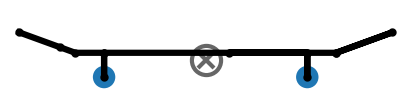
\includegraphics[]{paper/figure/Table1a.png}   
    & 0.876        & 5.002     & 18.885     & 2.377    & 0.122   & 1.778   & 1.430     & 0.266     & 2.261 
    & $l_{wb}=\SI{0.44}{\meter}$, $l_d=\SI{0.57}{\meter}$, \newline $l_t=\SI{0.13}{\meter}$, $\phi=\SI{20.0}{\degree}$, \newline $d_{tr}=\SI{0.053}{\meter}$, $r_w=\SI{0.024}{\meter}$ \\

    & & & & & & & & & & & \\

    Longboard   & 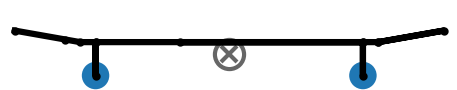
\includegraphics[]{paper/figure/Table1b.png}   
    & 0.604        & 3.638     & 11.321     & 3.277    & 0.250   & 0.952   & 1.289     & 0.089     & 1.304 
    & $l_{wb}=\SI{0.58}{\meter}$, $l_d=\SI{0.65}{\meter}$, \newline $l_t=\SI{0.14}{\meter}$, $\phi=\SI{10.0}{\degree}$, \newline $d_{tr}=\SI{0.073}{\meter}$, $r_w=\SI{0.030}{\meter}$ \\

    & & & & & & & & & & & \\

    Wheelbase   & 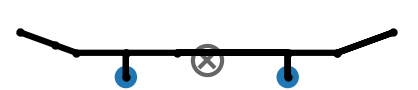
\includegraphics[]{paper/figure/Table1c.png}   
    & 0.899        & 4.618     & 19.288     & 2.377    & 0.104   & 2.228   & 1.453     & 0.302     & 2.427 
    & $l_{wb}=\SI{0.35}{\meter}$, $l_d=\SI{0.57}{\meter}$, \newline $l_t=\SI{0.13}{\meter}$, $\phi=\SI{20.0}{\degree}$, \newline $d_{tr}=\SI{0.053}{\meter}$, $r_w=\SI{0.024}{\meter}$ \\

    & & & & & & & & & & & \\

    Tail Length & 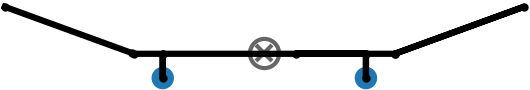
\includegraphics[]{paper/figure/Table1d.png}   
    & 0.855        & 4.972     & 15.398     & 2.979    & 0.257   & 4.038   & 1.399     & 0.227     & 2.092     
    & $l_{wb}=\SI{0.44}{\meter}$, $l_d=\SI{0.57}{\meter}$, \newline $l_t=\SI{0.30}{\meter}$, $\phi=\SI{20.0}{\degree}$, \newline $d_{tr}=\SI{0.053}{\meter}$, $r_w=\SI{0.024}{\meter}$ \\

    & & & & & & & & & & & \\

    Multiple Parameter & 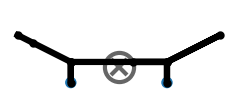
\includegraphics[]{paper/figure/Table1e.png}   
    & 0.982        & 5.073     & 42.762     & 1.459    & 0.020   & 2.856   & 1.509     & 0.338     & 2.569
    & $l_{wb}=\SI{0.21}{\meter}$, $l_d=\SI{0.21}{\meter}$, \newline $l_t=\SI{0.13}{\meter}$, $\phi=\SI{26.8}{\degree}$, \newline $d_{tr}=\SI{0.045}{\meter}$, $r_w=\SI{0.012}{\meter}$ \\
    
    \bottomrule
  \end{tabular}}
  \end{center}
    \caption[Results benchmarks]{Key values from the results of five different ollie optimizations: skateboards~1 and 2 are a fixed geometry popsicle skateboard and longboard respectively; skateboard~3 has an optimizable wheelbase; skateboard~4 has an optimizable tail/nose length; and skateboard~5 has an optimizable wheelbase, deck length, tail/nose inclination, truck height, and wheel radius. Mass centers are shown with a cross. ``Maximum human jump height'' is calculated by subtracting the take-off vertical position of the human's mass center from the maximum height of the human's mass center. The impact loss is calculated as the difference in skateboard kinetic energy before and after impact}
    \label{fig:resultstable}
\end{table*}

\begin{figure*}
    \centering
    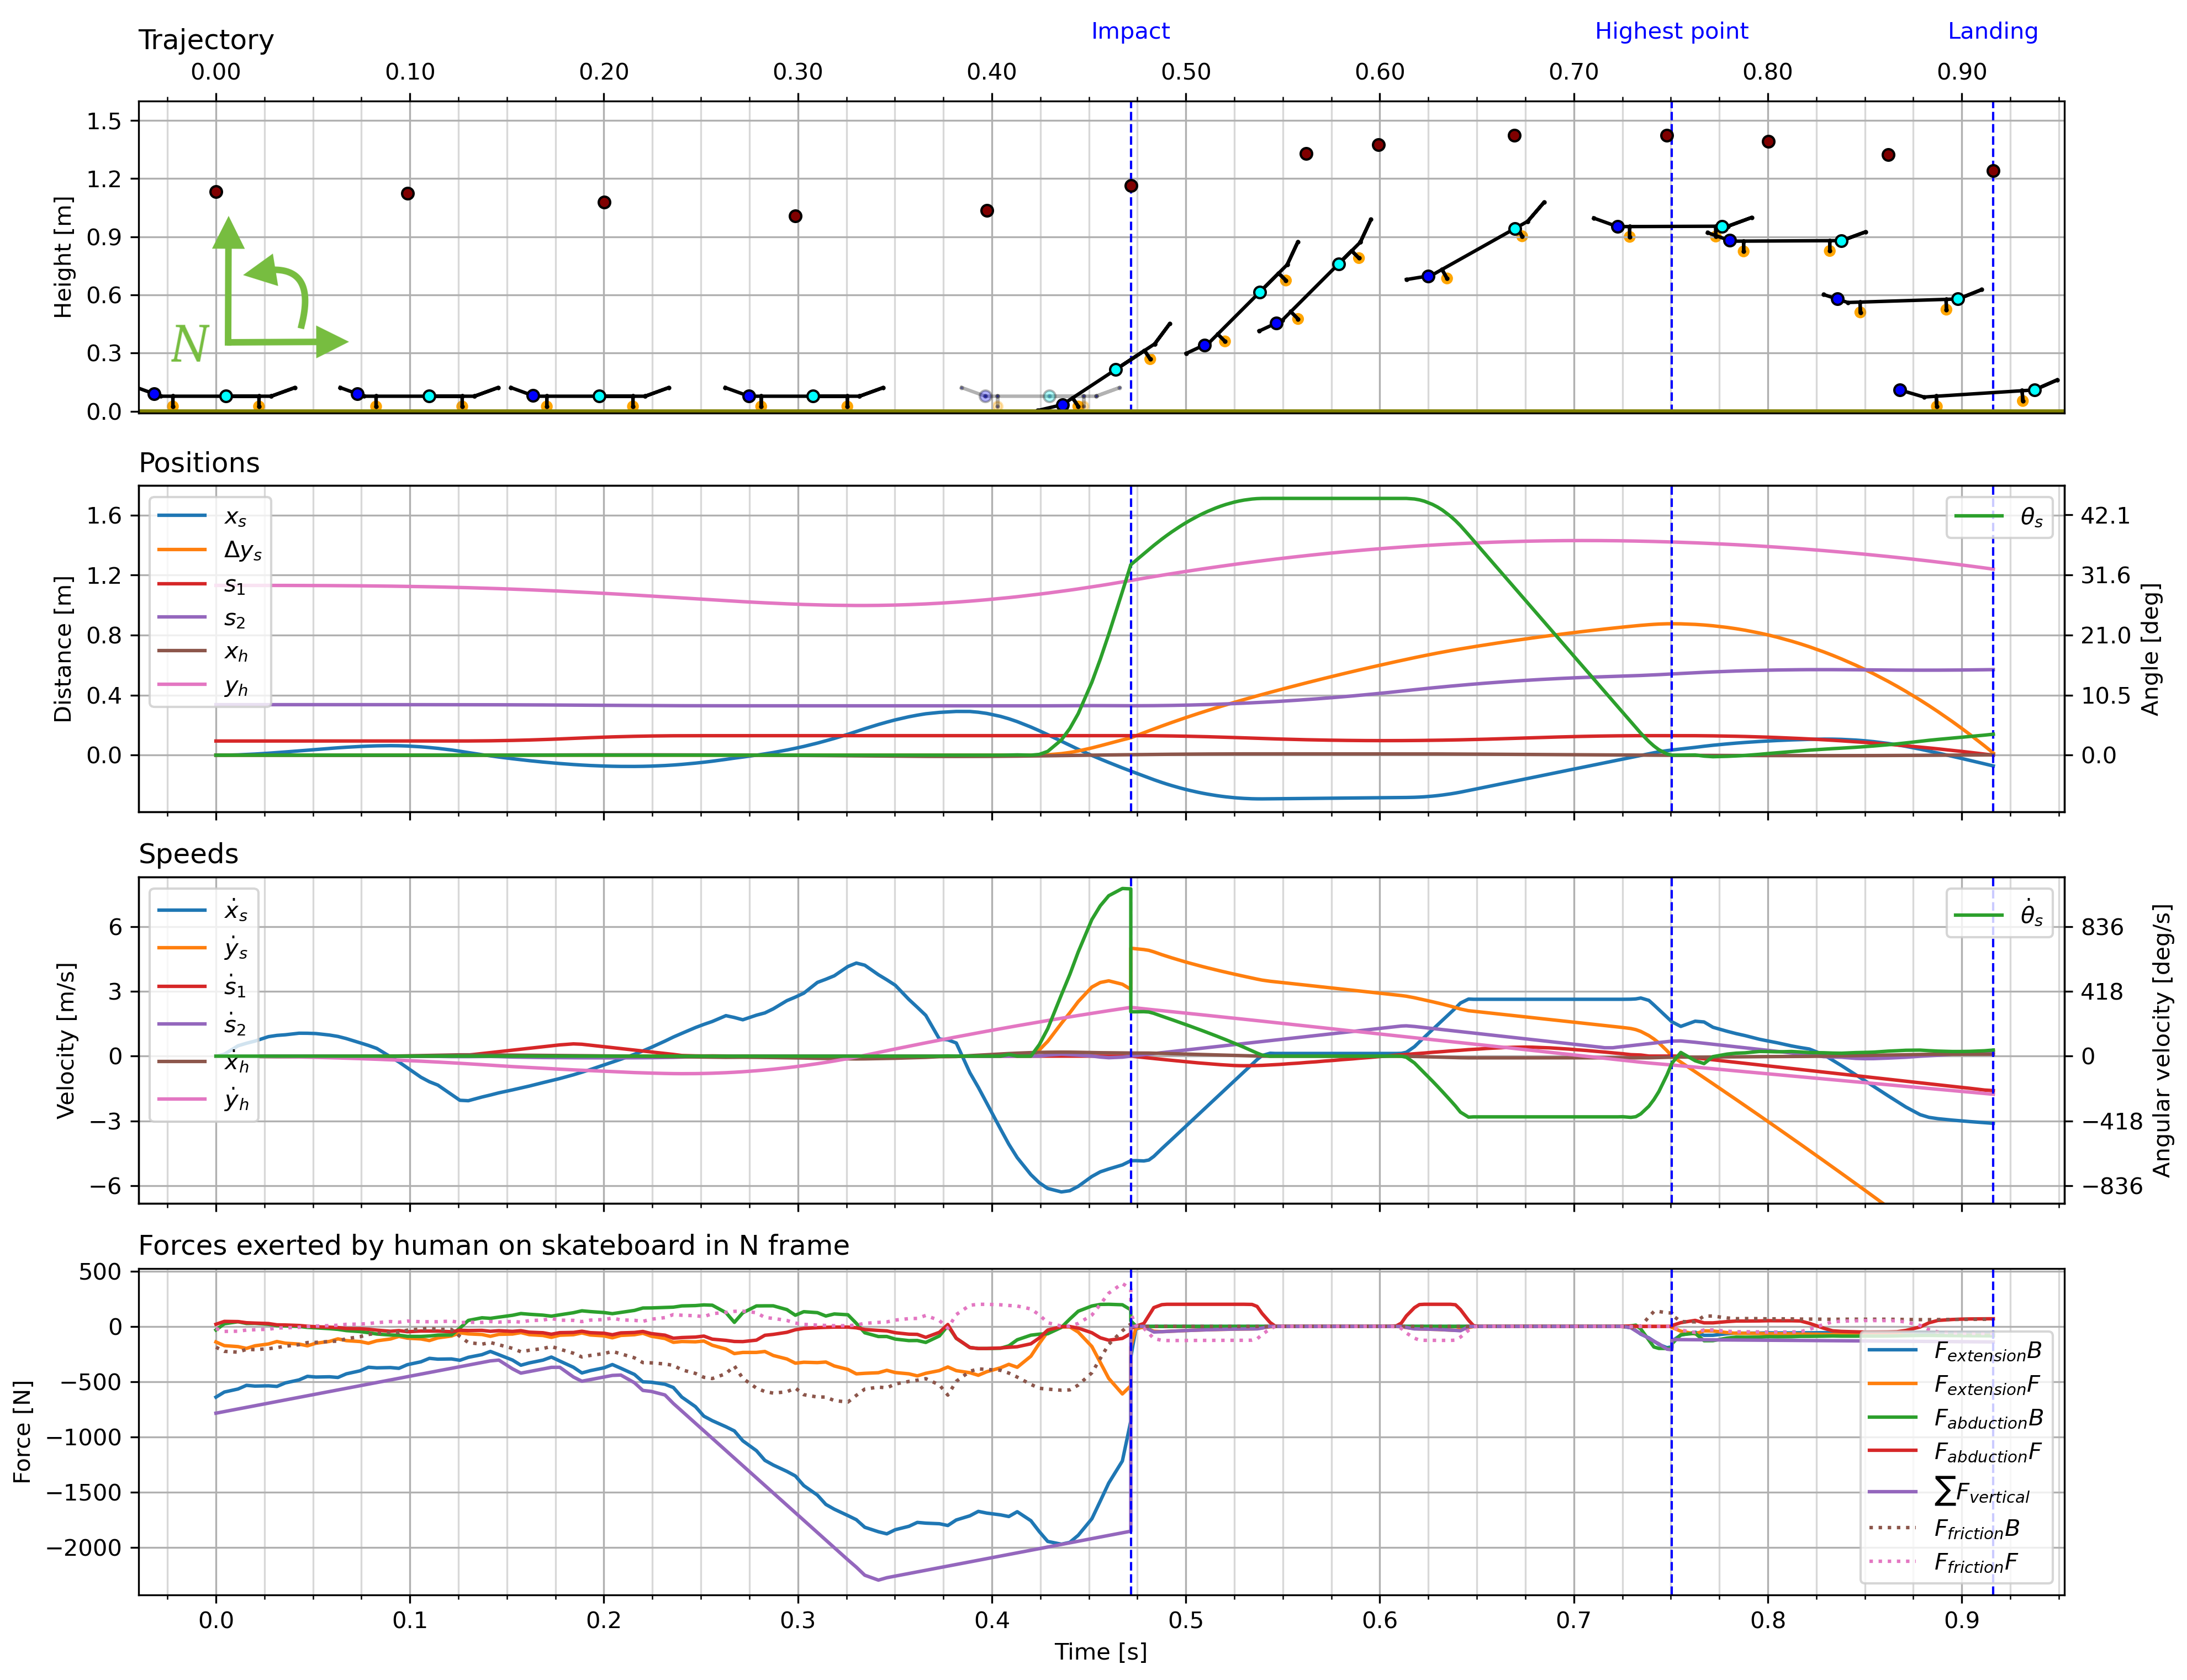
\includegraphics[trim={0cm 0cm 0cm 0cm},clip,width=\textwidth]{paper/figure/Fig6.png}
    \caption[Trajectory, positions, speeds, and forces of base optimization]{Detailed trajectory of base skateboard. The top subplot shows the trajectory of the skateboard relative to the human's mass center at various time instances. The second subplot shows the coordinates of the skateboard and the human. The third subplot shows the speeds of skateboard and human. The bottom subplot shows the extension ($N$-frame $y$-direction), abduction ($N$-frame $x$-direction), and sum of extension forces. The phase endpoints are shown by the vertical dotted blue lines}\label{f_noparameter}
\end{figure*}

\subsection{Base Skateboard Optimization}

The base skateboard optimal trajectory is shown in Fig.~\ref{f_noparameter} and is similar to the trajectory shown in Fig.~\ref{fig:ollie steps}.
Initially, the skateboard moves forward relative to the human. Immediately prior to the impact of the tail with the ground, the skateboard rapidly moves backward. 
The back foot initially moves to the pocket of the skateboard, the point with the lowest velocity of the tail during rotation.
Impact instantaneously changes the momentum of the skateboard.
In the speeds subplot of Fig.~\ref{f_noparameter} it is visible that the angular velocity reduces at impact (green line, \SIrange{1082}{286}{\degree\per\second}), while vertical velocity is gained (orange line, \SIrange{3}{5}{\meter\per\second}).

The human controller follows a countermovement jump force graph where unloading is from $t=\SIrange{0.0}{0.2}{\second}$, eccentric braking is at $t=\SIrange{0.2}{0.35}{\second}$, and the concentric phase is from $t=\SI{0.35}{\second}$ until impact.
During the concentric phase the vertical velocity (pink line) increases.
The force reduces to comply with the power bound ($P_{leg} = v_{rel} F$) until the human loses contact with the skateboard just before impact.
During upward motion, the vertical velocity of the human gradually decreases due to gravity, reaching its highest point just before the ollie's peak.
The slopes and maximum of the vertical forces (purple line) are bound by the eccentric (negative) and concentric (positive) rate of force development, and the maximum permitted force.
The optimizer operating at these bounds indicates that maximizing force and power output also maximizes ollie height.

\subsection{Longboard Optimization}
%
Despite similar force application to the longboard than those applied in the base \gls{ocp}, the maximum ollie height reduced by 31\%. This aligned with expectations as longboards are more challenging to ollie than popsicle stick skateboards in practice due to their larger size and can be explained by the lower translational and angular speeds achieved by this skateboard (Table~\ref{fig:resultstable}).

\subsection{Wheelbase Optimization}
%
\begin{figure*}
    \centering
    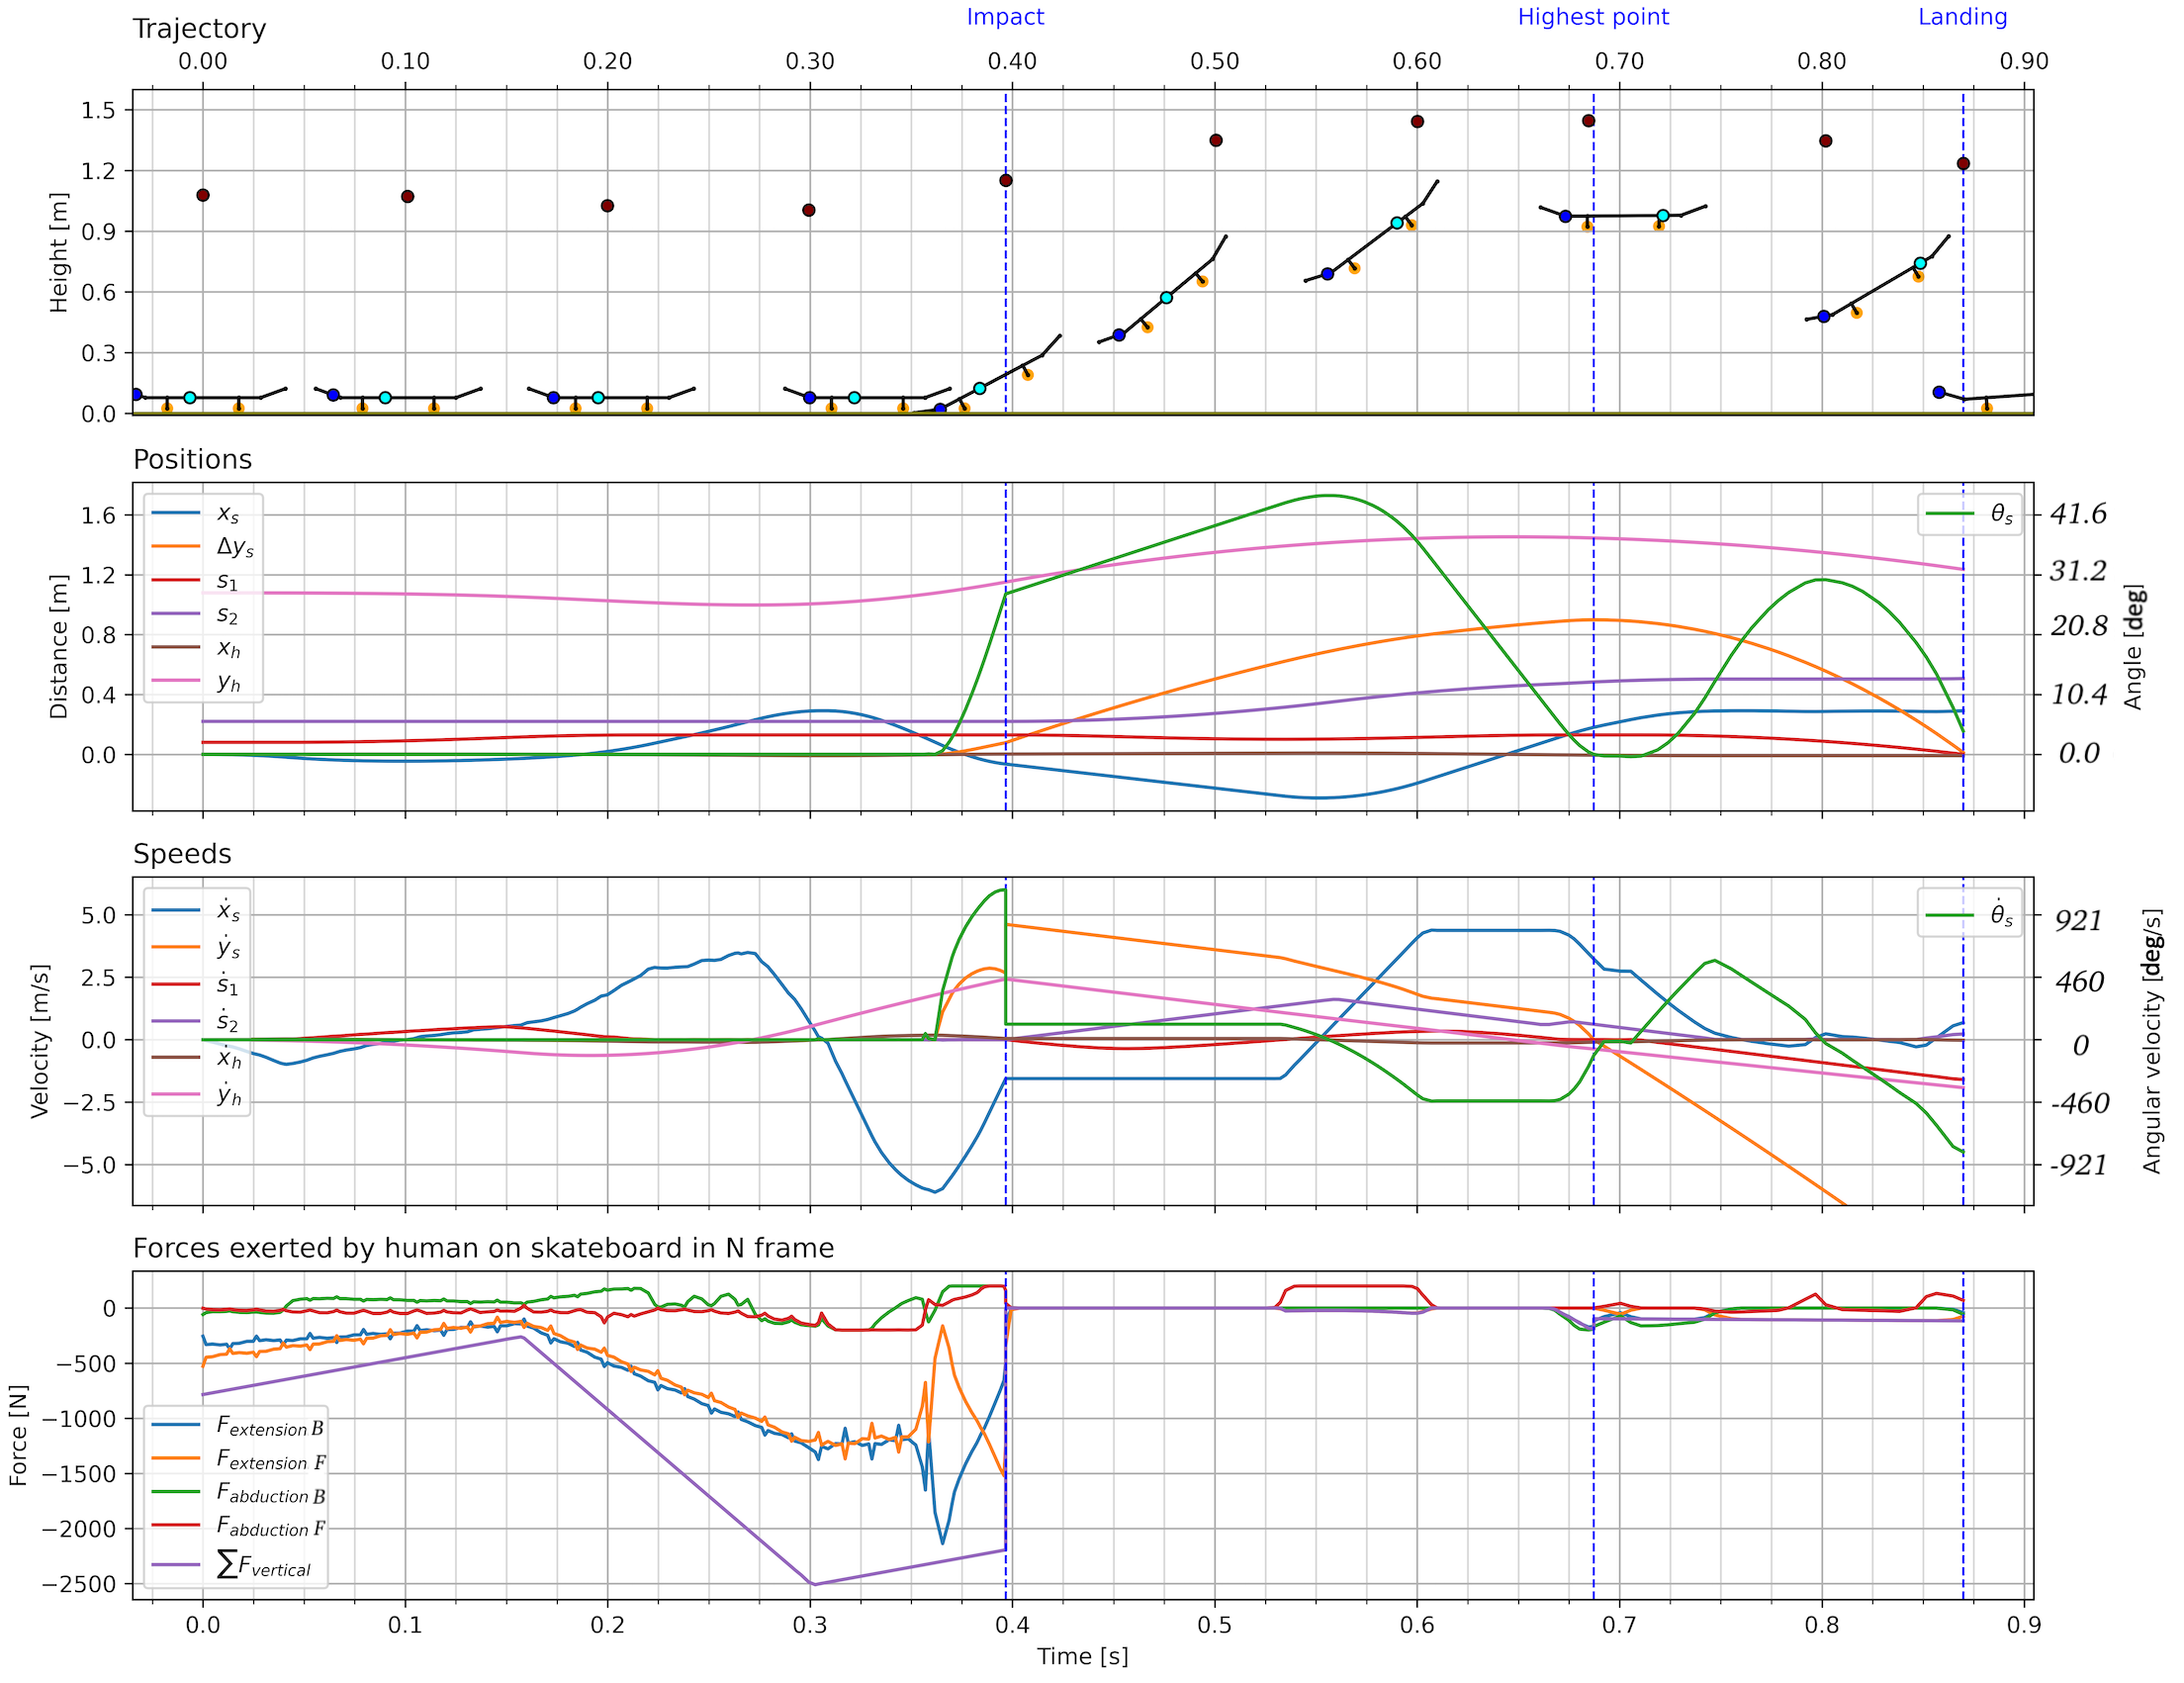
\includegraphics[trim={0cm 0cm 0cm 0cm},clip,width=\textwidth]{paper/figure/Fig7.png}    
    \caption[Trajectory, positions, speeds, and forces for wheelbase optimization]{Detailed trajectory of optimized wheelbase}\label{f_wheelbase}
\end{figure*}
\begin{figure*}
    \centering
    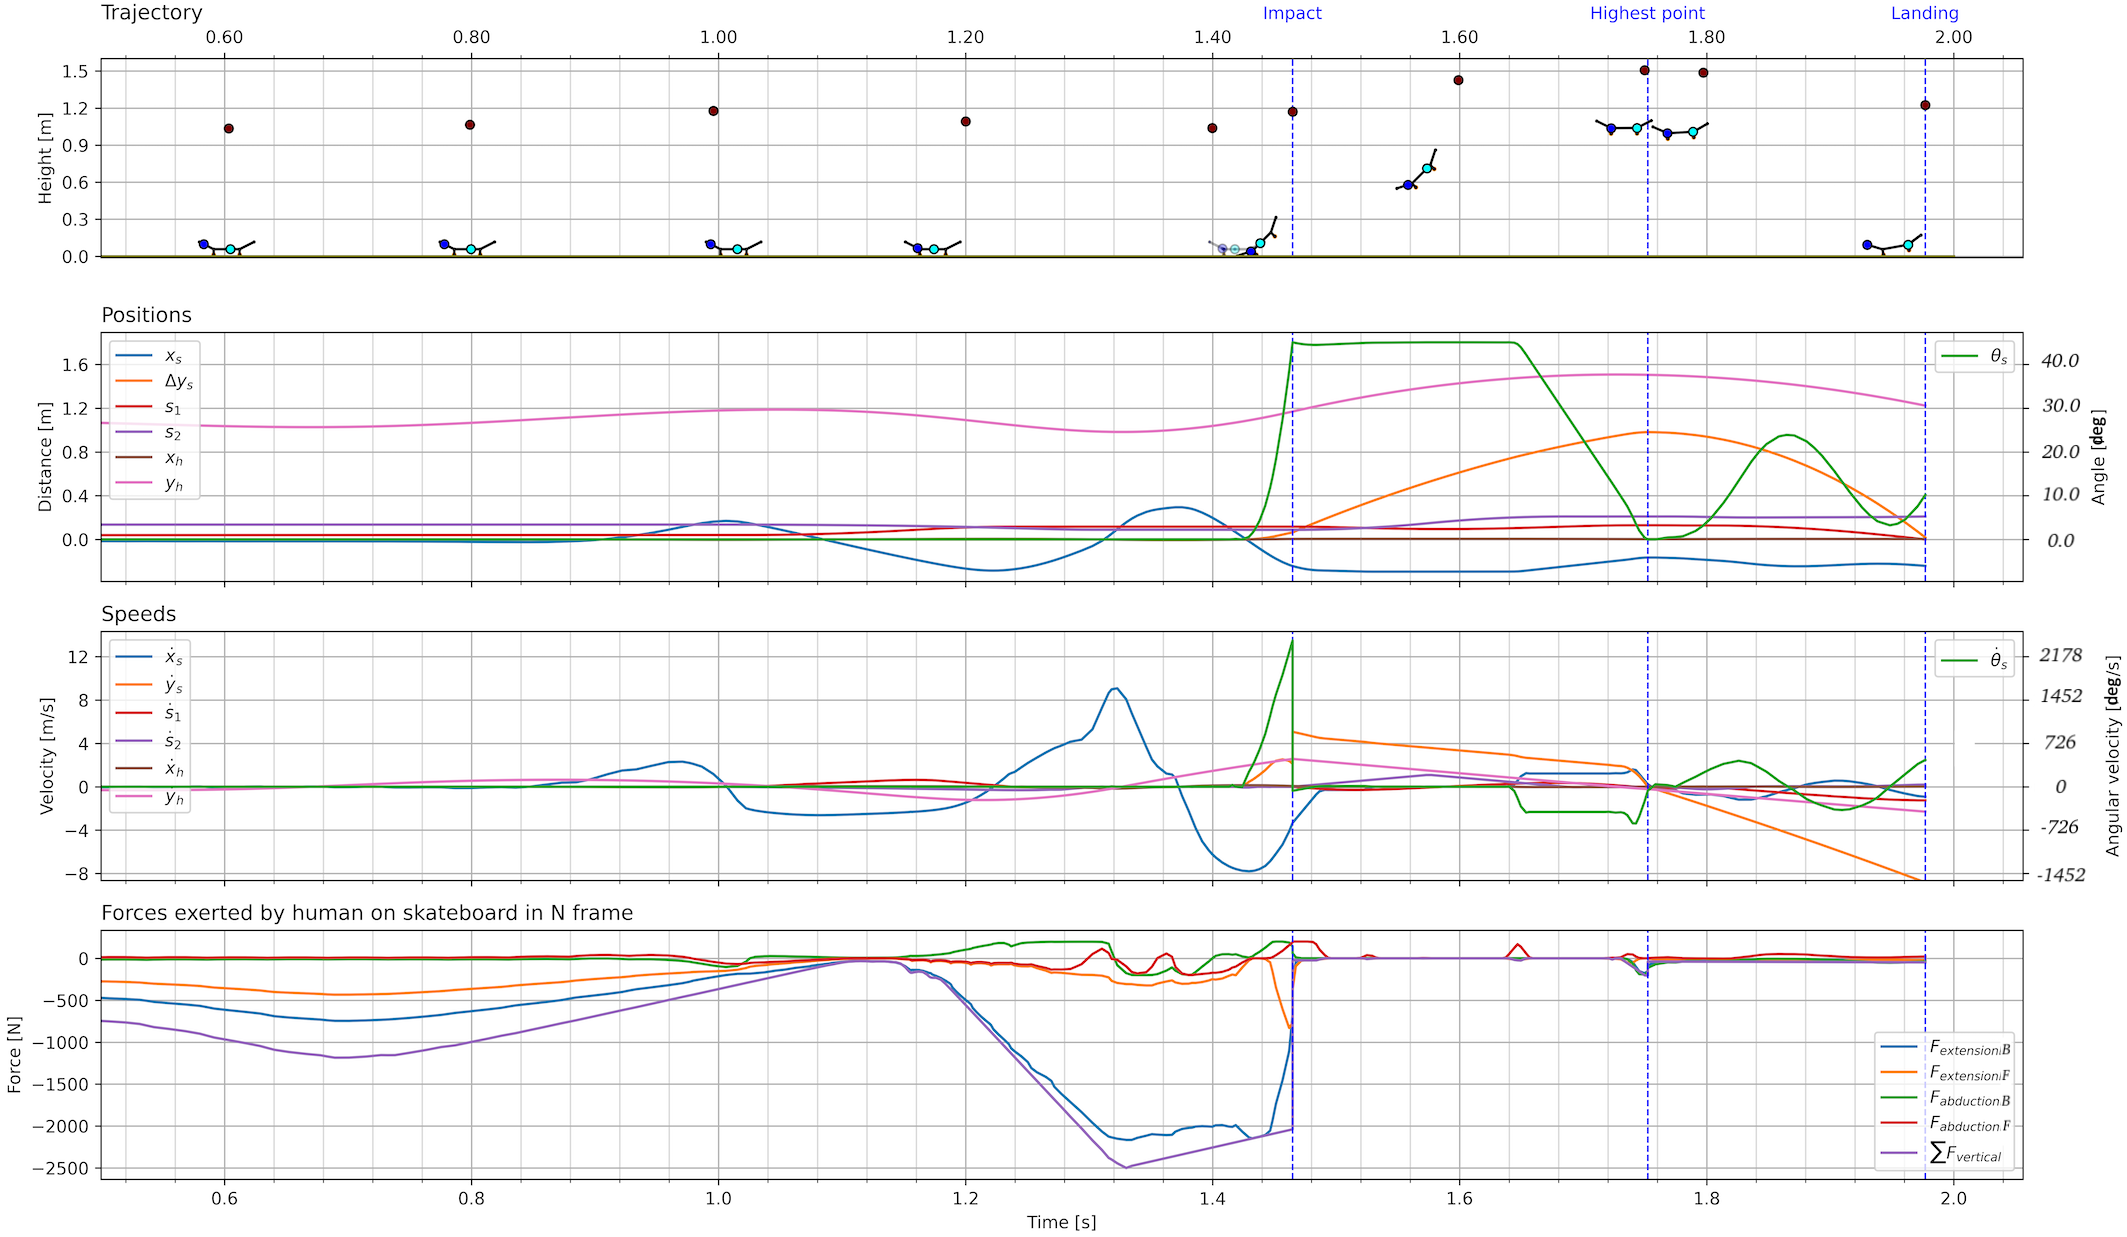
\includegraphics[trim={0cm 0cm 0cm 0cm},clip,width=\textwidth]{paper/figure/Fig8.png}
    \caption[Trajectory, positions, speeds, and forces for `all except tail length' optimization]{Detailed trajectory of optimization of all parameters except the tail}\label{f_notail}
\end{figure*}

In this \gls{ocp}, the wheelbase was reduced from \SIrange{0.44}{0.35}{\meter}, which allowed the peak ollie height to increase from \SIrange{0.876}{0.899}{\meter} (Table~\ref{fig:resultstable}).

Most of the phenomena seen in the results of the base \gls{ocp} are also visible for this \gls{ocp}.
The difference in ollie height can be attributed to the increased angular velocity for the shorter wheelbase board, which occurs for two reasons: more even distribution of force application pre-pop, and smaller impact angle.

The first difference is visible in the force subplot of Fig.~\ref{f_wheelbase}: the sum of the vertical forces (purple line) changes at its maximum rate during unloading and does not stagger like in Fig.~\ref{f_noparameter}.
The front and rear feet are equidistant from the rear wheel, allowing perfect balance.
In these positions, both legs can exert equal force without rotating the board during eccentric braking ($t=\SIrange{0.15}{0.30}{\second}$). 
Shortly before the impact, the front foot (orange line) releases pressure as the back foot pushes down to create maximal momentum about the back axis and a steep increase in angular velocity. 

The decreased wheelbase causes the impact angle to be lower and the angular velocity (green line) almost zero just after impact.
Consequently, no control is exerted while the skateboard gains height.
This is in contrast to the base skateboard \gls{ocp} solution, in which the front foot supplies an abduction force immediately after the pop.
Only a small downward force is applied to the skateboard at $t=\SI{0.53}{\second}$ to level it before the ollie's peak and fewer net vertical forces applied to the skateboard result in less vertical deceleration during its upward motion.

\subsection{Tail Length Optimization}
In solving the tail length \gls{ocp}, a maximum ollie height of \SI{0.855}{\meter} was found, in comparison to \SI{0.876}{\meter} for the base skateboard. Tail length was increased from \SIrange{0.14}{0.30}{\meter} (Table~\ref{fig:resultstable}). As the maximum ollie height is lower, the optimal solution is by definition a local minimum, a possible outcome.

\subsection{Multiple Parameter Optimization}
When five geometric parameters are free, the ollie height improves by \SI{0.106}{\meter} compared to the base skateboard and represents the highest ollie achieved by any optimized skateboard tested (Table~\ref{fig:resultstable}). 

This skateboard is significantly easier to rotate due to the lower inertia and mass ($I_s = \SI{0.02}{\kilo\gram\per\meter\squared}$ compared to $\SI{0.122}{\kilo\gram\per\meter\squared}$ and $m_s = \SI{1.459}{\kilo\gram}$ compared to $\SI{2.377}{\kilo\gram}$, seen in Table~\ref{fig:resultstable}).
With the same amount of force over time, the angular velocity (green line) is twice as high in comparison to the base skateboard solution.
The human also jumps highest with this skateboard setup.
With this setup, the skateboarder is able to jump almost solely from its back foot extension force (blue line) creating almost double the angular velocity as the other solutions (Fig.~\ref{f_notail}).

\section{Discussion}
The kinematics and kinetics of all ollies found as a result of the \glspl{ocp} resemble the motion and strategy used in real ollies.
Without any motion cues, the optimization successfully replicates the ollie motion, with almost all phenomena seen in Fig.~\ref{fig:ollie steps}.
The solutions show that it is optimal for the human to first jump, then slam the skateboard tail into the ground, then slide the front foot over the deck to drag it up and level it out, and finally catch (stop) the skateboard with the back foot at the skateboard's highest point.
All results also show high similarities to a countermovement jump ground reaction force.
The sum of the human control forces naturally bound to realistically produced values and rates due to the model constraints.
In an ollie ground reaction force, the impulse from the skateboard hitting the ground is roughly \SI{5}{\joule}~\cite{determan_kinetics_2006}, which is of the same order of magnitude as the found impact losses in Table~\ref{fig:resultstable}.
Based this and our anecdotal motion comparisons, our simple ollie model may be useful for insights in the ollie dynamics, human kinetic output, and human movement.

Lower inertia and skateboard mass are beneficial for ollie height.
Comparing the solutions for the base skateboard and longboard we see an expected trend that ollie height decreases (by 31\%) for the larger board.
In all parameter optimizations that improved ollie height compared to the base skateboard, a reduction in mass and inertia is found.
This makes sense dynamically because it is easier to lift and rotate the skateboard if it has less mass and inertia, yet our model does not illuminate the fine motor skills relative to foot size needed to ollie such a board. Thus a very small board may not be an optimum in reality.

A standard popsicle stick skateboard is close to optimum and slight changes in its geometry do not influence the ollie height significantly.
This implies that skaters can make small modifications to skateboard geometry without significantly penalizing ollie height.
The best performing single parameter optimization was only able to ollie \SI{0.023}{\meter} higher than the base skateboard.
When multiple parameters are changed the ollie height increased significantly by 12\%.
However, the geometry and size of the resulting skateboard were significantly different from a popsicle stick skateboard.
Skaters will also need to consider tricks other than the ollie and likely therefore keep the popsicle stick skateboard as the norm. Our optimizations have not yet revealed small realizable changes that can  significantly improve ollie height.
But if ollie height were the only consideration, it could likely be improved by drastically changing the skateboard.
Out of the six single parameters tested~\cite{heinen_optimal_2022}, ollie height is most improved by the wheelbase.
Shortening the wheelbase could be a promising area of further investigation since it does not influence the board shape, which is crucial for other tricks.

We have developed a new contact implicit friction model compatible with generalized \gls{ocp}s by restating the hybrid relaxed formulation of \citet{patel_contact-implicit_2019} using a simplified contact definition.
Static and dynamic friction is achieved while retaining the ability to have contact implicit events.
The simplification leads to quicker convergence and works with a null seed initial guess.
The ollie \gls{ocp} by \citet{shield_contact-implicit_2022} was without any parameter optimization. Theirs took 43 minutes to solve and needed accurate initial guesses to achieve convergence.
All \glspl{ocp} using our formulation solved in under 3 minutes, which includes the time taken to derive the \glspl{eom} and all constraints, and transcribe and solve the \gls{ocp}.
Furthermore, this was all done without an accurate initial guess, which is known to be beneficial for not biasing the \gls{ocp} solution~\cite{betts_practical_2010}.

Parameter optimization of tail length leads to a local maximum.
Tail length is maximized despite this resulting in a lower ollie height.
In reality, a longer tail length would cause a higher energy dissipation due to it bending more during impact.
A plausible cause for this local maximum is that impact loss is of too little effect.
When a human jumps, the order of magnitude of the amount of energy necessary to go up is on the order of $10^3\si{\joule}$ ($mgh=100\si{\kilo\gram}\cdot10\si{\meter\per\second\squared}\cdot1\si{\meter}$). The dissipation of energy during impact is on the order of $10^{-1}\si{\joule}$.
This means that the impact loss has such a limited effect on increasing ollie height that the solution space is likely very flat.
The model does capture the increase in impact loss in Table~\ref{fig:resultstable}, but it is not sufficient to influence the solution. Higher fidelity models that provide more links from board properties to human motion could improve this.
All other solutions are not guaranteed to be global optima either as direct collocation does not guarantee finding a global optimum.
Though, finding higher outcomes than the base optimization is still valuable for interpreting performance through geometrical dimensions.

In future research, we advise to implement a normal force acting on the front wheel during the preparation phase.
The front foot also has to counteract the rotation created by the back foot. 
In reality, the front foot could be located anywhere forward of the rear truck without causing a counterclockwise rotation due to the compensation of the normal force.
This could also be a reason why the force curves are not completely smooth; the board must balance on the rear wheel prior to the pop.

\section{Conclusions}
In this paper, we formulate and efficiently solve an \gls{ocp} that simultaneously finds the human-applied time-varying control force and optimal board geometry to perform a maximal height skateboard ollie without any prescribed motion cues. Our model is designed to be simple, yet able to capture the essential dynamics of this complex human-board maneuver. The lumped point mass model of the human based on the countermovement jump ensures that the forces delivered to the skateboard are realistically bound in magnitudes and rates. Both board-ground impact and foot-board friction are utilized when executing an ollie. Our formulation makes both of these discontinuous model elements compatible with the direct collocation discretization scheme. In particular, we introduce a new simplified contact implicit friction model that improves the convergence properties of the \glspl{ocp}, enabling 10 times faster \gls{ocp} solve times than similar problems and more robust convergence from less accurate initial guesses.

The resulting simulations show qualitatively and quantitatively similar motions to real ollies. The maximal achievable heights reflect expected geometric changes to the board, i.e. increased mass and inertia result in lower ollies, giving credence that our objective function is sound. We learned that simply decreasing the wheelbase may result in higher ollies, without affecting the other geometry of the board. Yet, small changes to geometry do not seem to result in large changes to ollie height. When optimizing for multiple geometric parameters, the optimizer chooses a small board and strategy that maximizes the angular velocity at tail impact to give an ollie 12\% higher than the base board design.

This model and the results provide a new stone in the foundation needed for utilizing optimization to improve skateboard trick strategy and performance. In its current form, it can be used to inform jump strategy and the effects of changes to the essential board geometry. Tying this tool to experimental studies of skateboard ollies is an obvious next research step.

\section{Acknowledgments}
None

\section{Statements and Declarations}

\subsection{Supplementary Information}
%
Animations of the solutions are included as supplementary material.

\subsection{Data availability}
%
The software used to generate the optimal control solutions is available at \url{https://github.com/mechmotum/ollie-optimization}.

\subsection{Conflicts of Interest}
%
There has been no conflict of interest with the
authors involved in this work.

\bibliographystyle{sn-basic}
\bibliography{references}

\end{document}